\typeout{IJCAI-16 Instructions for Authors}

\documentclass{article}
% The file ijcai16.sty is the style file for IJCAI-16 (same as ijcai07.sty).
\usepackage{ijcai16}

% Use the postscript times font!
\usepackage{times}

% the following package is optional:
%\usepackage{latexsym} 

% author added packages
\usepackage{xspace}
\usepackage{graphicx}
\usepackage{epsfig}
\usepackage{array}

\newcommand{\ispy}{\textit{I, Spy}\xspace}
\newcommand{\examplepicsize}{0.075}
\newcommand{\pictablew}{0.6in}

%\title{Grounded Attribute Learning with Multi-Modal Perception}
\title{Learning Multi-Modal Grounded Linguistic Semantics by Playing \ispy}
\author{Paper XXX}
%\author{name \\ 
%affiliation  \\
%email}

\begin{document}

\maketitle

\begin{abstract}
% The abstract should be no more than 200 words long
Grounded language learning bridges human language words like `red' and `square' with robot perception.
The vast majority of existing work in this space limits perception to robot vision.
In this paper, we build perceptual models that use haptic, auditory, and proprioceptive data acquired through robot exploratory behaviors that go beyond vision alone.
Our system learns to ground natural language predicates about objects using supervision from an interactive human-robot \ispy game.
In this game, the human and robot take turns describing an object on a table, then trying to guess which object the other has described.
All predicate labels were gathered from human subjects physically present to play this game with an embodied robot.
We demonstrate that our multi-modal system for grounding natural language outperforms a traditional, vision-only grounding framework by comparing the two on the \ispy task.
We also provide a qualitative analysis of the predicates learned in the game, visualizing groups of predicates that can be understood from the same kinds of robot perception and pointing out predicates for which vision alone is insufficient (e.g. `empty').
\end{abstract}

\section{Introduction}
\label{sec:introduction}
	Robots need to be able to connect language to their environment in order to discuss real world objects with humans.
Mapping from referring expressions such as ``the blue cup'' to their object referents in the world is part of the \textit{symbol grounding problem}~\cite{harnad:phys90}.
Symbol grounding involves connecting internal representations of information in a machine to real world data from its sensory perception.
\textit{Grounded language learning} bridges these symbols with natural language.

Early work on grounded language learning enabled a machine to map between adjectives and nouns such as ``red'' and ``block'' to objects in a scene through vision-based classifiers~\cite{roy:evocomm01}.
We refer to adjectives and nouns that describe properties of objects as language \textit{predicates}.
Most work has focused on grounding language predicates through visual information. However, other sensory modalities such as haptic and auditory are also useful in allowing robots to discriminate between objects~\cite{sinapov:icra14}.
This paper explores grounding language predicates by considering visual, haptic, auditory, and proprioceptive senses. 

A home or office robot can explore objects in an unsupervised way to gather perceptual data, but needs human supervision to connect this data to language.
Learning grounded semantics through natural human-robot dialog allows a system to acquire the relevant knowledge without the need for laborious labeling of numerous objects for every potential lexical descriptor.
A few other groups have explored learning from interactive linguistic games such as \ispy and ``20 Questions'' \cite{parde:ijcai15,vogel:aaai10}; however, these studies have been restricted to simple objects and only employed vision (see Section \ref{sec:relatedwork}).

\begin{figure}
\centering
\begin{tabular}{c}
	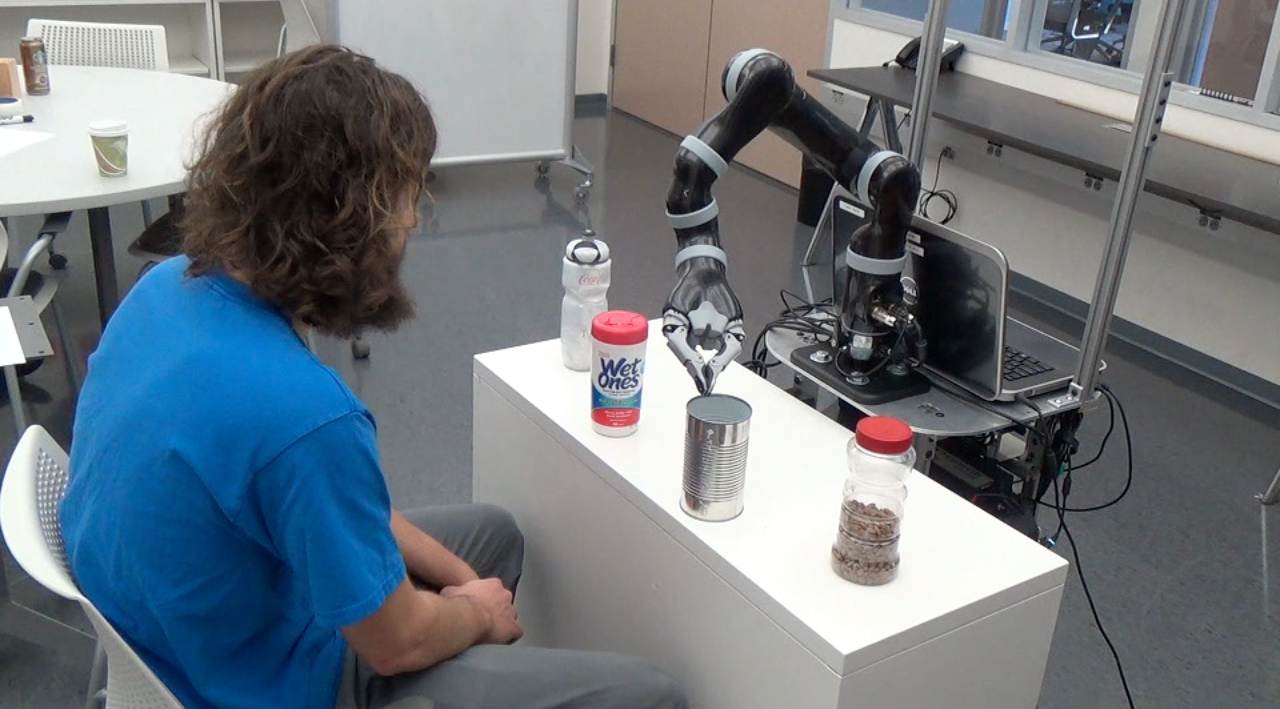
\includegraphics[width=0.3\textwidth]{figures/silver_round_and_empty.png} \\
	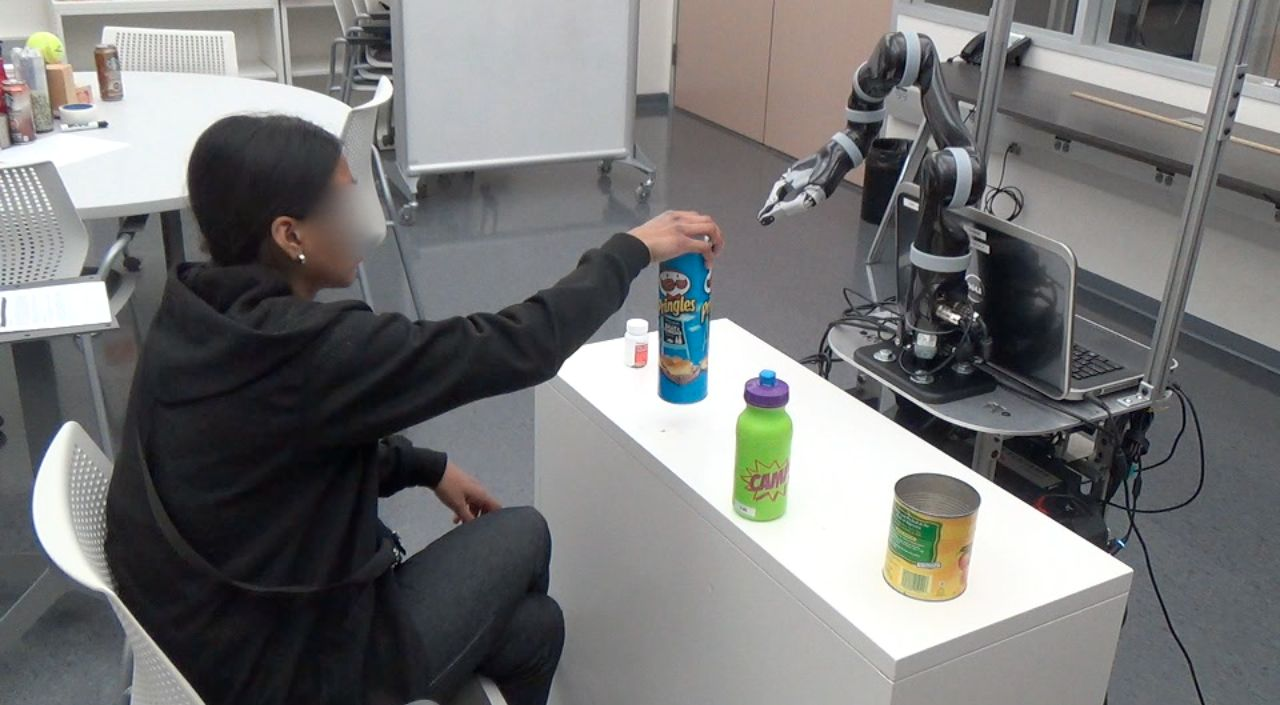
\includegraphics[width=0.3\textwidth]{figures/light_tall_tub.jpg} \\
\end{tabular}
\caption{\textbf{Top}: the robot guesses an object described by a human subject as ``silver, round, and empty.'' \textbf{Bottom}: a human subject guesses an object described by the robot as ``light,'' ``tall,'' and ``tub.''}
\label{fig:ispy}
\end{figure}

We use a variation on the children's game \ispy, as a learning framework for gathering human language labels for objects to learn multi-modal grounded lexical semantics.
Figure~\ref{fig:ispy} shows the players (humans and the robot) guessing an object the other has described.
Our experimental results test generalization to new objects not seen during training and illustrate both that the system learns accurate word meanings and that modalities beyond vision improve its performance.

To our knowledge, this is the first robotic system to perform natural language grounding using multi-modal sensory perception through feedback with human users.

\section{Related Work}
\label{sec:relatedwork}
	% relation to grounded language learning tasks
Researchers have made substantial progress on grounding language for robots, enabling tasks like object recognition and route following from verbal descriptions. 
Early work used vision together with speech descriptions of objects for this learning~\cite{roy:cogsci02}.

In the past few years, much of this work has focused on combining language with visual information. 
For grounding referring expressions in an environment, many learn perceptual classifiers for words like `red', `square', and `left' given some pairing of human descriptions and labeled scenes~\cite{liu:acl14,malinowski:nips14,mohan:acs13,sun:icra13,dindo:iros10,vogel:aaai10}. 
Some works additionally incorporate language models into the learning phase~\cite{spranger:ijcai15,krishnamurthy:acl13,perera:aaai13,matuszek:icml12}. 
Our method uses simple language understanding and constructs new attribute classifiers for new, unseen words used by a human playing \ispy. 
Unlike any previous methods, our classifiers take advantage of more than just visual data from objects.

Including a human in the learning loop provides a more realistic learning scenario for applications such as household robotics. 
Past work has used human speech plus gestures describing sets of objects on a table as supervision to learn attribute classifiers~\cite{matuszek:aaai14,kollar:rss13}. 
Recent work introduced the \ispy game as a framework for supervision~\cite{parde:ijcai15} for grounded language learning. 
Outside of robotics, there has been some work on combining language with other sensory modalities than vision, such as audio~\cite{kiela:emnlp15}. 
Our work differs from these in that we use experience gathered from more than vision to build object attribute classifiers. 
In our instantiation of the \ispy task, the robot and the human both take a turn describing objects, where in previous work~\shortcite{parde:ijcai15} only the human played this role. 
To our knowledge, ours is the first work to integrate visual, haptic, auditory, and proprioceptive information for language grounding by an embodied robot.

% relation to multi-modal perception (i.e. jivko's work)
% TODO: jivko

\section{Task Definition}
\label{sec:taskdefinition}
	In our \ispy task, the human and robot take turns describing objects from among four on a tabletop [[Figure picture??]].
There are two rounds of turns in each game. In each round, the human subject starts by describing and object of her choice.

Subjects were asked to describe objects through their attributes, as opposed to singling them out as instances.
As an example, we suggested subjects describe an object as ``black rectangle'' as opposed to ``whiteboard eraser.''
Additionally, subjects were told they could handle the objects physically before offering a description, but were not asked to use non-visual predicates.
Once subjects offered a description, the robot guessed the objects it most thought the subject was talking about in order (see section~\ref{ssec:gll}) until one was confirmed correct.

In the second half of each round, the robot picked an object and then described it with up to three predicates (see section~\ref{ssec:gll}).
The subject was again able to pick up and physically handle objects before guessing.
The robot confirmed or denied each subject guess  until the right object was chosen.

The \ispy game admits two clear metrics.
The \textit{robot guess} metric is the number of turns the robot took to guess what object the subject was describing.
The \textit{human guess} metric is the number of turns the human took to guess what object the robot was describing.
Using these metrics, we compare the performance of two \ispy playing systems as described in section ~\ref{sec:experiment}.

\section{Dataset}
\label{sec:dataset}
	\begin{figure}
\centering
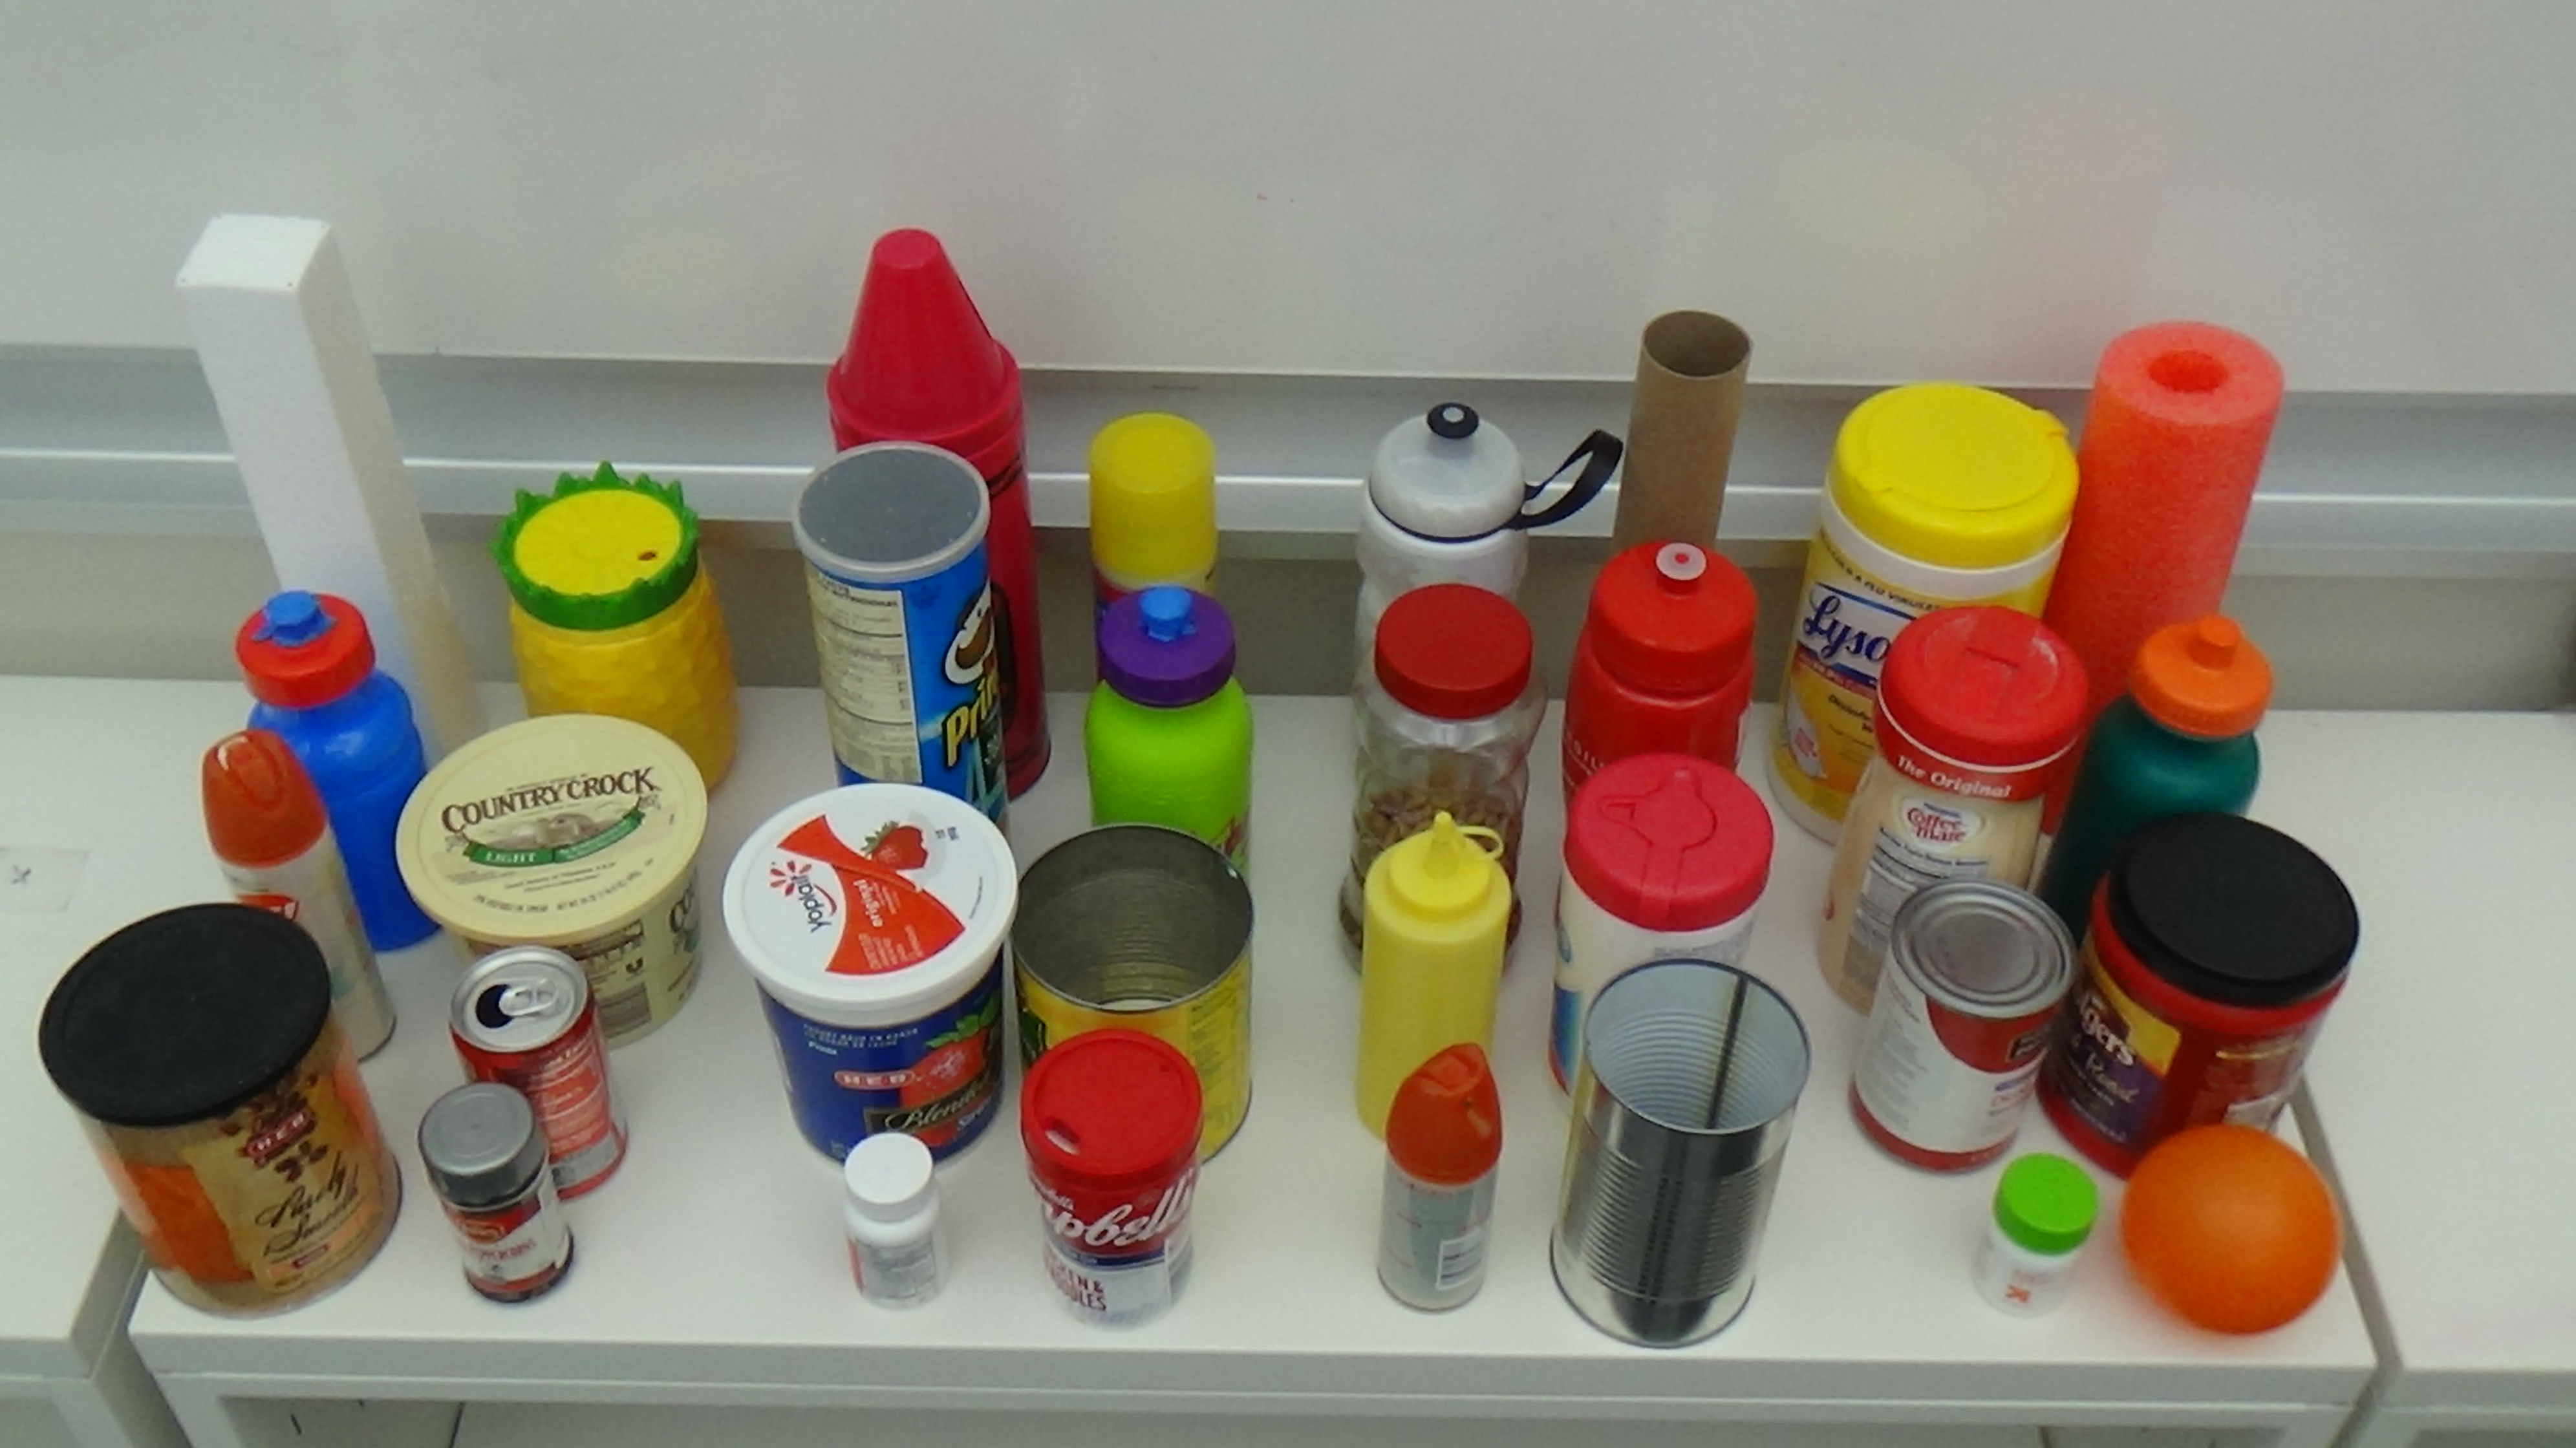
\includegraphics[width=0.3\textwidth]{figures/objects.jpg}
\caption{Objects used in the \ispy game divided into the four folds discussed in Section~\ref{ssec:methodology}, from fold 0 on the left to fold 3 on the right.}
\label{fig:objects}
\end{figure}

The robot used in this study was a Kinova MICO arm mounted on top of a custom-built mobile base, which remained stationary during our experiment.
The robot's sensors included joint effort sensors in each of the robot arm's motors, a microphone mounted on the mobile base, and the Xtion ASUS Pro RGBD camera.
The set of objects used in this experiment consisted of 32 common household items including cups, bottles, cans, and other containers, shown in Figure~\ref{fig:objects}.
Some of the objects contained liquids or other contents (e.g., coffee beans) while others were empty.
Contemporary work gives a more detailed description of this object dataset~\cite{sinapov:ijcai16}, but we briefly describe the exploration and modalities below.

\subsection{Exploratory Behaviors and Sensory Modalities}
\label{ssec:contexts}

\begin{center}
\begin{figure}[t]
\setlength{\unitlength}{1in}
 \centerline{
\begin{picture}(3.5,2.5)
\put(0.0,1.4){\psfig{file=figures/behaviors/grasp1.eps,width=1.1in}}
\put(0.4,1.275){grasp}
\put(1.2,1.4){\psfig{file=figures/behaviors/lift1_arrow.eps,width=1.1in}}
\put(1.7,1.275){lift}
\put(2.4,1.4){\psfig{file=figures/behaviors/lower1_arrow.eps,width=1.1in}}
\put(2.8,1.275){lower}
\put(0.0,0.075){\psfig{file=figures/behaviors/drop1.eps,width=1.1in}}
\put(0.45,-0.05){drop}
\put(1.2,0.075){\psfig{file=figures/behaviors/press1_arrow.eps,width=1.1in}}
\put(1.6,-0.05){press}
\put(2.4,0.075){\psfig{file=figures/behaviors/push2_arrow.eps,width=1.1in}}
\put(2.8,-0.05){push}
\end{picture}
}
\caption{The behaviors the robot used to explore the objects.
The arrows indicate the direction of motion of the end-effector for each behavior.
In addition, the {\it hold} behavior (not shown) was performed after the {\it lift} behavior by simply holding the object in place for half a second.}
\label{fig:behaviors}
\end{figure}
\end{center}
\vspace {-5mm}

Prior to the experiment, the robot explored the objects using the methodology described by Sinapov et al.~\shortcite{sinapov:ras14}, and the dimensionality of the raw auditory, haptic, and proprioceptive data were reduced comparably (final dimensionality given in Table~\ref{tab:feature_space_of_contexts}).
In our case, the robot used 7 distinct actions: {\it grasp}, {\it lift}, {\it hold}, {\it lower}, {\it drop}, {\it push}, and {\it press}, shown in Figure~\ref{fig:behaviors}.
During the execution of each action, the robot recorded the sensory perceptions from {\it haptic} (i.e., joint efforts) and {\it auditory} sensory modalities.
During the {\it grasp} action, the robot recorded {\it proprioceptive} (i.e., joint angular positions) sensory information from its fingers.
The joint efforts and joint positions were recorded for all 6 joints at 15 Hz.
The auditory sensory modality was represented as the Discrete Fourier Transform computed using 65 frequency bins.

In addition to the 7 interactive behaviors, the robot also performed the {\it look} action prior to grasping the object which produced three different kinds of sensory modalities: 1) an RGB color histogram of the object using 8 bins per channel; 2) Fast point feature histogram ({\it fpfh}) shape features~\cite{rusu:icra09} as implemented in the Point Cloud Library~\cite{aldoma:ram12}; and 3) deep visual features from the 16-layer VGG network~\cite{simonyan:corr14}.
The first two types of features were computed using the segmented point cloud of the object while the deep features were computed using the 2D image of the object. 

\begin{table}
\centering
\begin{tabular}[h]{|l|c|c|c|}
	\hline
	\bf Behavior & \multicolumn{3}{c|}{\bf Modality} \\ \hline \hline
	& \bf color & \bf fpfh & \bf vgg \\ \hline
	\bf look & 64 & 308 & 4096 \\ \hline \hline
	& \bf audio & \bf haptics & \bf proprioception \\ \hline
	\bf grasp & 100 & 60 & 20 \\ \hline
	\bf drop, hold, & & & \\
	\bf lift, lower, & 100 & 60 & \\
	\bf press, push & & & \\ \hline
\end{tabular}
\caption{The number of features extracted from each \textit{context}, or combination of robot behavior and perceptual modality.}
\label{tab:feature_space_of_contexts}
\end{table}

Thus, each of the robot's 8 actions produced two to three different kinds of sensory signals.
Each viable combination of an action and a sensory modality is a unique sensorimotor context.
In our experiment, the set of contexts $\mathcal{C}$ was of size  $2 \times 3 + 6 \times 2 = 18$.
The robot performed its full sequence of exploratory actions on each object 5 different times (for the {\it look} behavior, the object was rotated to a new angle each time). Given a context $c \in \mathcal{C}$ and an object $i \in \mathcal{O}$, let the set $\mathcal{X}_i^c$ contain all five feature vectors observed with object $i$ in context $c$.

\section{Implementation}
\label{sec:implementation}
	To play \ispy, we first gathered sensory data from the set of objects through robot manipulation behaviors (described in Section~\ref{sec:dataset}).
When playing a game, the robot was given unique identifying numbers for each object on the table and could look up relevant feature vectors when performing grounding.

During the course of the game, the robot used its RGBD camera to detect the locations of the objects and subsequently detect whenever a human reached out and touched an object in response to the robot's turn.
The robot could also reach out and point to an object when guessing.
We implemented robot behaviors in the Robot Operating System\footnote{\texttt{http://www.ros.org/}} and performed text-to-speech using the Festival Speech Synthesis System.\footnote{\texttt{http://www.cstr.ed.ac.uk/projects/festival/}}

	\subsection{Multi-Modal Perception}
	\label{ssec:mmp}
	For each language predicate $p$, a classifier $G_p$ was learned to decide whether objects possessed the attribute denoted by $p$.
This classifier was informed by sub-classifiers that determined whether $p$ held for a particular subset of the features used to describe objects.

The feature space of objects was partitioned according contexts, as discussed in Section~\ref{ssec:contexts}.
Each context classifier $M_{c}, c\in\mathcal{C}$ is a quadratic-kernel SVM trained with positive- and negative-labels for context feature vectors derived from the \ispy game (Section~\ref{ssec:gll}).
Then $M_{c}(\mathcal{X}_i^c)\in [-1,1]$, the average classifier output over all observations for object $i\in\mathcal{O}$ where individual SVM decisions on observations were in $\{-1,1\}$.

Following previous work in multi-modal exploration~\cite{sinapov:icra14}, for each context we calculated the Cohen's Kappa $\kappa_{c}$ to measure the agreement across observations between the decisions of the $M_{c}$ classifier and the ground truth labels from the \ispy game, in order to serve as a confidence in $[0,1]$ for each context
\footnote{We use $\kappa$ instead of accuracy because we can expect most objects to be negative examples of a given predicate. $\kappa$ better handles such skewed-class data than accuracy, which could be deceptively high for a classifier that always returns false.}.
We ceiling negative $\kappa$ to $0$.

Given these context classifiers and associated confidences, we calculate an overall decision, $G_p(i)$, for $i\in\mathcal{O}$ for each behavior $b$ and modality $m$ as:
\begin{equation}
	G_p(i) = \sum_{c\in\mathcal{C}}{\kappa_{c} M_{c}(\mathcal{X}_i^c)} \in [-1,1]
\end{equation}
The sign of $G_p(i)$ gives a decision on whether $p$ applies to $i$ with confidence $|G_p(i)|$.


	\subsection{Grounded Language Learning}
	\label{ssec:gll}
	Language predicates and positive/negative labels for those predicates were gathered through human-robot dialog during the \ispy game.
The human subject and robot were seated at opposite ends of a small table.
A set of 4 objects were placed on the table for both to see.
We denote the objects on the table during a given game as set $\mathcal{O}_T$.

\paragraph{Human Turn.} On the subject's turn, the robot asked him or her to pick an object and describe it in one phrase.
We used a standard stopword list to strip out non-content words from the subject's description.
The remaining words were treated as a set of language predicates, $\mathcal{H}_p$.
The robot assigned scores $S$ to each object $i\in \mathcal{O}_T$ on the table.
\begin{equation}
	S(i) = \sum_{p\in \mathcal{H}_p}{G_p(i)}
\end{equation}
The robot guessed objects in descending order by score (ties broken randomly) by pointing at them and asking whether it was correct.
When the correct object was found, it was added as a positive training example for all classifiers  $p\in \mathcal{H}_p$ for use in future training.

\paragraph{Robot Turn.} On the robot's turn, an object was chosen at random from those on the table.
To describe the object, the robot scored the set of known predicates learned from previous play.
Following Gricean principles~\cite{grice:bkchapter75}, the robot attempted to describe the object with predicates that applied to it but did not ambiguously refer to other objects on the table.
We use a predicate score $R$ that rewards describing the chosen object $i^*$ and penalizes describing the other objects on the table.
\begin{equation}
	R(p) = |O_T|D_p(i^*) - \sum_{j\in{\mathcal{O}_T}\setminus\{i^*\}}{D_p(j)}
\end{equation}
Note that this scoring equation also rewards predicates for describing $i^*$ while clearly {\it not} describing the other objects on the table (\textit{e.g.}  $D_p(j)<0$).
The robot choose up to three highest scoring predicates $\hat{P}$ to describe object $i^*$ to the subject, using fewer if $S<0$ for remaining predicates.
Once ready to guess, the subject touched objects until the robot confirmed that they had guessed the right one ($i^*$).

The robot then pointed to $i^*$ and engaged the user in a brief follow-up dialog in order to gather both positive and negative labels for $i^*$.
In addition to predicates $\hat{P}$ used to describe the object, the robot selected two additional predicates $\bar{P}$.
$\bar{P}$ were selected randomly with $p\in P$ having a chance of inclusion proportional to $1-|G_p(i^*)|$, such that classifiers with low confidence in whether or not $p$ applied to $i^*$ were more likely to be selected.
The robot then asked the subject whether they would describe the object $i^*$ using each $p\in\hat{P}\cup\bar{P}$.
The subject's responses to these questions provided additional positive/negative labels to the classifiers of these predicates for use in future training.


\section{Experiment}
\label{sec:experiment}
	To determine whether multi-modal perception helps a robot perform well in a grounding task, we had two systems play \ispy with 40 human subjects.
The baseline \textbf{vision only} system used only the \textbf{look} behavior when grounding language predicates, analogous to many past works as discussed in section~\ref{sec:relatedwork}.
Our \textbf{multi-modal} system used the full suite of behaviors and associated haptic, proprioceptive, and auditory modalities shown in Table~\ref{tab:feature_space_of_contexts} when grounding language predicates.

	\subsection{Methodology}
	\label{ssec:methodology}
	\paragraph{Data Folds.}
We divided our 32-object dataset into 8 folds.
For each fold, at least 10 human subjects played \ispy with both the \textbf{vision only} and \textbf{multi-modal} systems (12 subjects in the final fold).
Four games were played by each subject.
The \textbf{vision only} system and \textbf{multi-modal} system were each used in two games (once as a the describer and once as the guesser), and their temporal order was randomized.
Each system played with all 8 objects, but the split and the order of objects on the table were randomized.

For fold 0, the systems were undifferentiated and so only one set of two games was played by each subject. 
For subsequent folds, the systems were incrementally trained using labels from previous folds only, such that the systems were always being tested against novel, unseen objects.
In the prior work using the \ispy game~\cite{parde:ijcai15}, the same objects were used during training and test, and therefore it did not test the ability of the learned predicate classifiers to actually generalize to novel objects.

\paragraph{Human Subjects.}

Our 42 subjects were undergraduate and graduate students as well as some staff at our university.

At the beginning of each trial, subjects were shown an instructional video of one of the authors playing a single game of \ispy with the robot, then given a sheet of instructions about the task's turn-taking and how to communicate with the robot. 
In every game, subjects took one turn and the robot took one turn.

A study coordinator remained in the room to deal with system mechanical and software failures, both of which resulted in the current game starting over.
To avoid noise from automatic speech recognition, the study coordinator also transcribed the subject's speech to the system from a remote computer, but this was done discretely and not revealed to the subject until debriefing when the games were over.


	\subsection{Quantitative Results}
	\label{ssec:results}
	To determine whether our \textbf{multi-modal} approach outperformed a traditional \textbf{vision only} approach, we measured the average number of robot guesses and human guesses in games played with each fold of objects.
The systems were identical in fold 0 since both were untrained.
In the end, we trained the systems on all available data to calculate predicate classifier agreement with human labels.

\begin{figure}
\centering
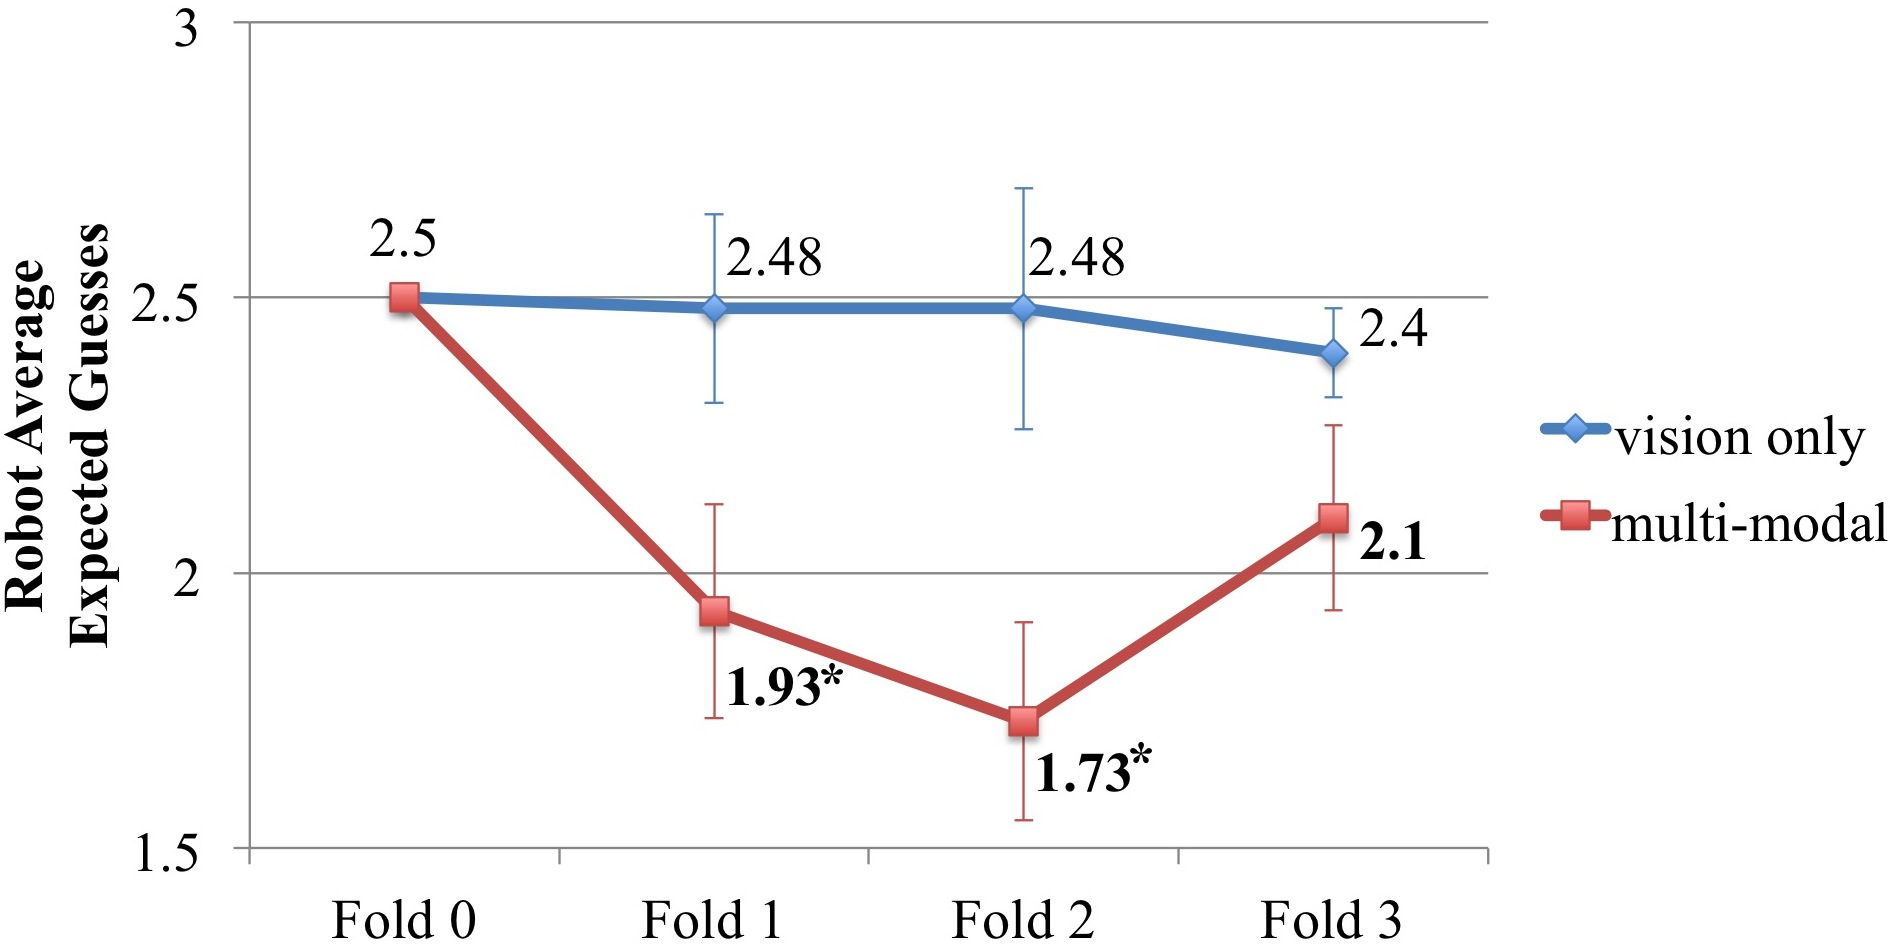
\includegraphics[width=0.5\textwidth]{figures/robot_guesses_error_bars.jpg}
\caption{Average expected number of guesses the robot made on each human turn with standard error bars shown.
\textbf{Bold}: significantly lower than the average at fold 0 with $p<0.05$ (unpaired Student's $t$-test).
\textbf{*}: significantly lower than the competing system on this fold on participant-by-participant basis with $p<0.05$ (paired Student's $t$-test).}
\label{fig:robot_guesses}
\end{figure}

\textbf{Robot guess.} Figure~\ref{fig:robot_guesses} shows the average number of robot guesses for the games in each fold. Because we had access to the scores the robot assigned each object, we calculated the {\it expected} number of robot guesses for each turn.
For example, if all 4 objects were tied for first, the expected number of robot guesses for that turn was 2.5, regardless of whether it got (un)lucky and picked the correct object (last)first.\footnote{2.5 is the expected number for 4 tied objects because the probability of picking in any order is equal, so the expected turn to get the correct object is $\frac{1+2+3+4}{4} = \frac{10}{4} = 2.5$}

After training on just one fold, our \textbf{multi-modal} approach performs statistically significantly better than the expected number of turns for guessing (the strategy for the untrained fold 0 system) for the remainder of the games.
The \textbf{vision only} system, by contrast, is never able to differentiate itself significantly from random guessing, even as more training data becomes available.
We suspect the number of objects is too small for the \textbf{vision only} system to develop decent models of many predicates, whereas \textbf{multi-modal} exploration allows that system to extract more information per object.

\textbf{Human guess.} Neither the \textbf{vision only} nor \textbf{multi-modal} system's performance improves on this metric with statistical significance as more training data is seen.
Human guesses hovered around 2.5 throughout all levels of training and sets of objects.

This result highlights the difficulty of the robot's turn in an \ispy framework, which requires not just good coverage of grounded words (as when figuring out what object the human is describing), but also high accuracy when using classifiers on new objects.
Context classifiers which had few examples could achieve confidence $\kappa=1$, making the predicates they represented more likely to be chosen to describe objects.
It is possible that the system would have performed better on this metric if the predicate scoring function $R$ additionally favored predicates with many examples.

\textbf{Predicate Agreement.} Training the predicate classifiers using leave-one-out cross validation over objects, we calculated the average precision, recall, and $F_1$ scores of each against human predicate labels on the held-out object.
Table~\ref{tab:predicate_results} gives these metrics for the 74 predicates used by the systems.\footnote{There were 53 predicates shared between the two systems.
The results in Table~\ref{tab:predicate_results} are similar for a paired $t$-test across these shared predicates with slightly reduced significance.}

\begin{table}
\centering
\begin{tabular}[h]{|l|r|r|}
	\hline
	\bf Metric & \multicolumn{2}{c|}{\bf System} \\ \hline \hline
	& \bf vision only & \bf multi-modal \\ \hline
	precision & .250 & .378\textbf{+} \\
	recall & .179 & .348\textbf{*} \\
	\bf $F_1$ & .196 & .354\textbf{*} \\ \hline
\end{tabular}
\caption{Average performance of predicate classifiers used by the \textbf{vision only} and \textbf{multi-modal} systems in leave-one-object-out cross validation.
\textbf{*}: significantly greater than competing system with $p<0.05$.
\textbf{+}: $p<0.1$ (Student's un-paired $t$-test).}
\label{tab:predicate_results}
\end{table}

Across the objects our robot explored, our \textbf{multi-modal} system achieves consistently better agreement with human assignments of predicates to objects than does the \textbf{vision only} system.


	\subsection{Qualitative Results}
	\label{ssec:qualitative}
	We explored the predicates learned by our systems qualitatively, looking at the differences in individual predicate classifier agreements, the objects picked out by these classifiers in each system, and correlations between predicate decisions and objective measurements of object qualities such as weight and height.

\paragraph{When multi-modal helps.}
To determine when the \textbf{multi-modal} system's non-visual information helped make good decisions, we did a pairwise comparison of predicates built in the \textbf{multi-modal} and \textbf{vision only} systems.
Table~\ref{tab:predicate_examples} shows the predicates for which the difference in $\kappa$ between the two systems was high and there were enough objects with labels that these confidences were nontrivial.

\begin{table*}
\centering
\begin{tabular}[t]{| c | c || >{\centering\arraybackslash}m{\pictablew} | >{\centering\arraybackslash}m{\pictablew} | >{\centering\arraybackslash}m{\pictablew} || >{\centering\arraybackslash}m{\pictablew} | >{\centering\arraybackslash}m{\pictablew} | >{\centering\arraybackslash}m{\pictablew} |}
	\hline
	\bf Predicate & $\kappa_{mm}-\kappa_{vo}$ & \multicolumn{3}{c||}{\bf High Confidence Positive} & \multicolumn{3}{c|}{\bf High Confidence Negative} \\ \hline \hline
	\multicolumn{2}{|c|}{} & \multicolumn{6}{c|}{\bf multi-modal system} \\ \hline
	can & 1 & 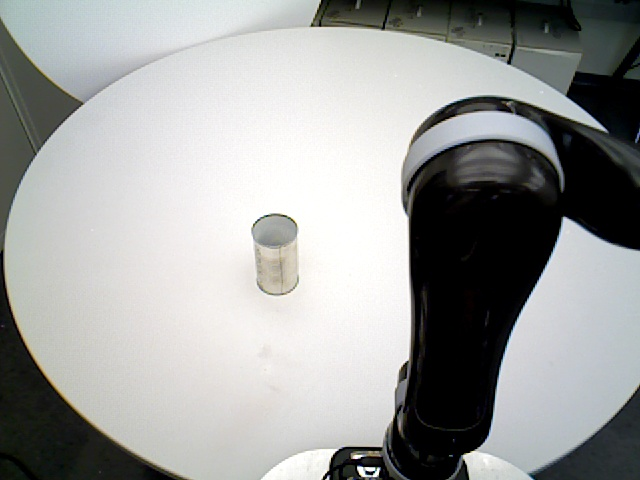
\includegraphics[scale=\examplepicsize]{figures/objects/9.JPG} & 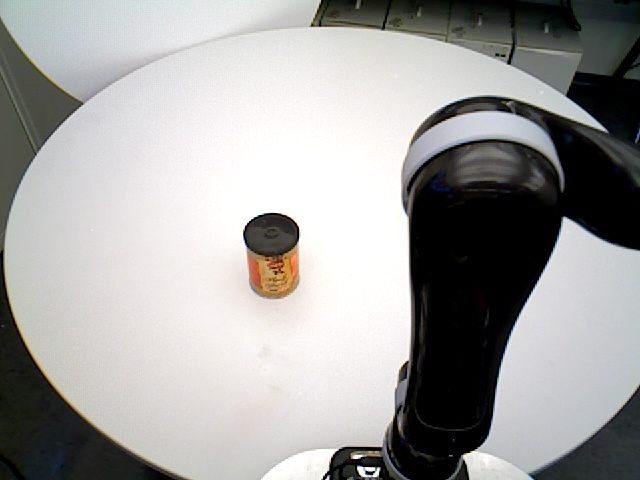
\includegraphics[scale=\examplepicsize]{figures/objects/3.JPG} & 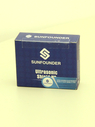
\includegraphics[scale=\examplepicsize]{figures/objects/6.JPG} & 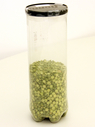
\includegraphics[scale=\examplepicsize]{figures/objects/28.JPG} & 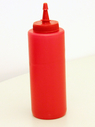
\includegraphics[scale=\examplepicsize]{figures/objects/21.JPG} & 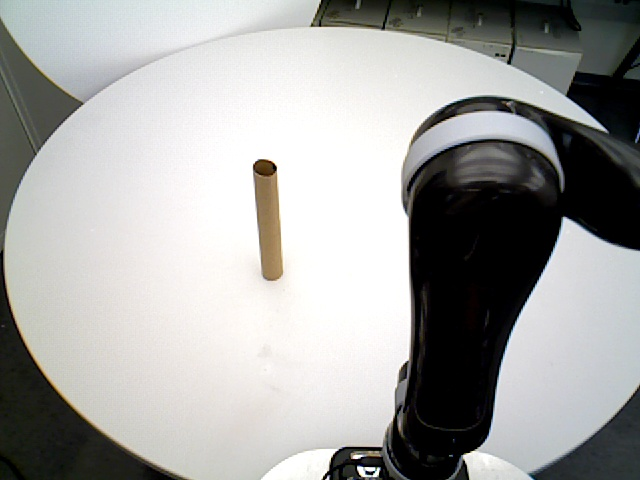
\includegraphics[scale=\examplepicsize]{figures/objects/4.JPG}\\ \hline
	tub & 1 & 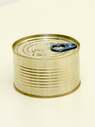
\includegraphics[scale=\examplepicsize]{figures/objects/30.JPG} & 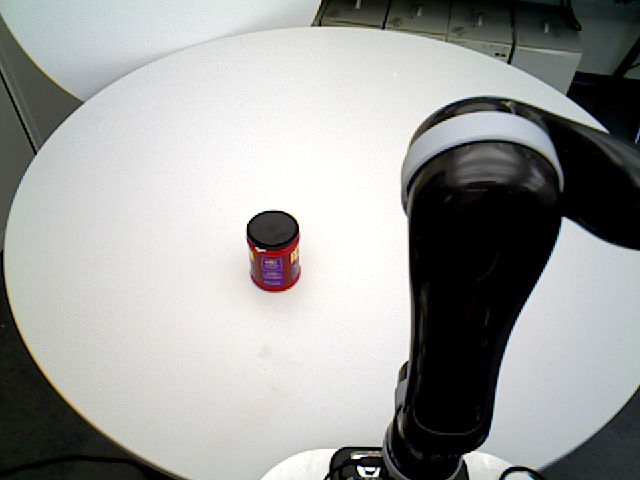
\includegraphics[scale=\examplepicsize]{figures/objects/10.JPG} & 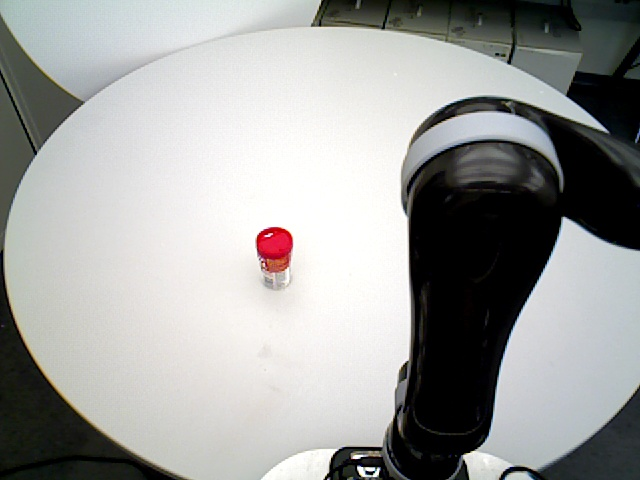
\includegraphics[scale=\examplepicsize]{figures/objects/11.JPG} & 
\includegraphics[scale=\examplepicsize]{figures/objects/14.JPG} & 
\includegraphics[scale=\examplepicsize]{figures/objects/2.JPG} & 
\includegraphics[scale=\examplepicsize]{figures/objects/18.JPG}\\ \hline
	empty & .637 & 
\includegraphics[scale=\examplepicsize]{figures/objects/14.JPG} & 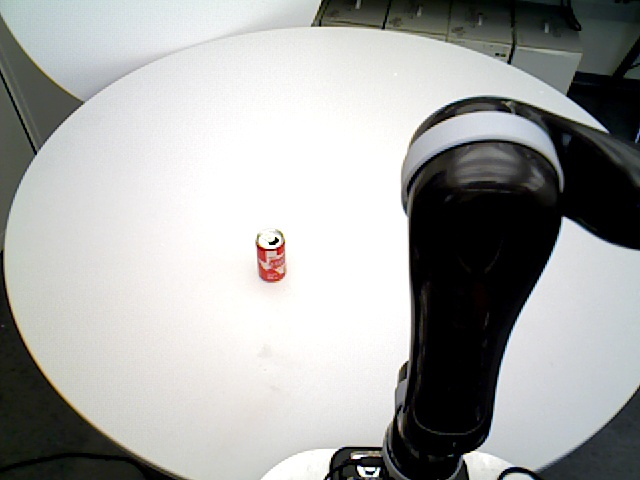
\includegraphics[scale=\examplepicsize]{figures/objects/27.JPG} & 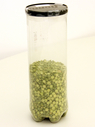
\includegraphics[scale=\examplepicsize]{figures/objects/28.JPG} & 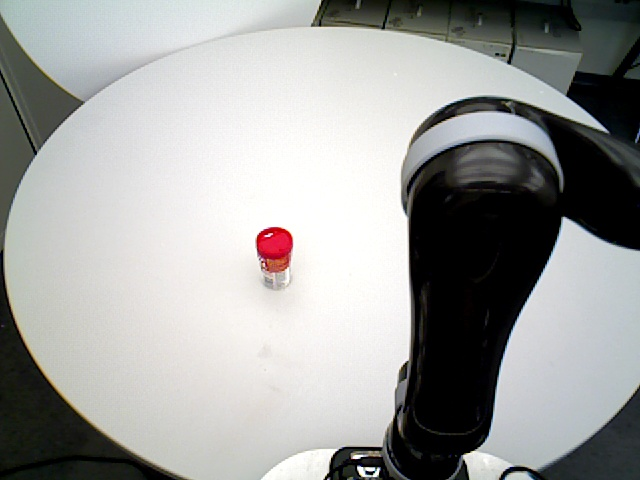
\includegraphics[scale=\examplepicsize]{figures/objects/11.JPG} & 
\includegraphics[scale=\examplepicsize]{figures/objects/31.JPG} & 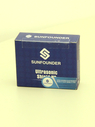
\includegraphics[scale=\examplepicsize]{figures/objects/6.JPG}\\ \hline
	tall & .566 & 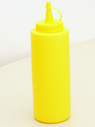
\includegraphics[scale=\examplepicsize]{figures/objects/19.JPG} & 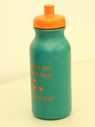
\includegraphics[scale=\examplepicsize]{figures/objects/24.JPG} & 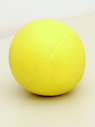
\includegraphics[scale=\examplepicsize]{figures/objects/25.JPG} & 
\includegraphics[scale=\examplepicsize]{figures/objects/15.JPG} & 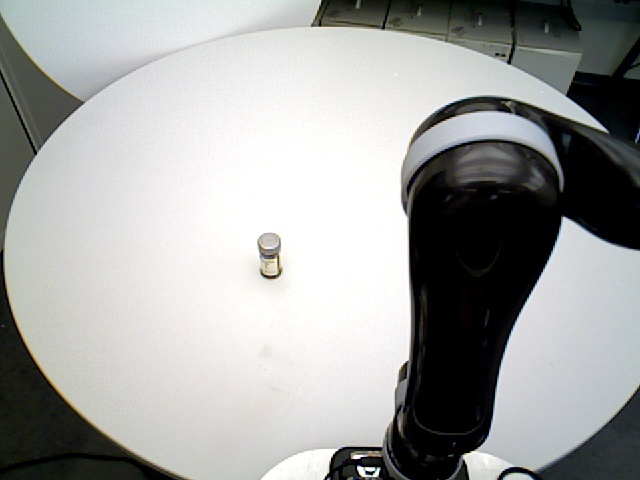
\includegraphics[scale=\examplepicsize]{figures/objects/26.JPG} & 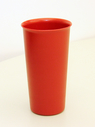
\includegraphics[scale=\examplepicsize]{figures/objects/7.JPG}\\ \hline
	\multicolumn{2}{|c|}{} & \multicolumn{6}{c|}{\bf vision only system} \\ \hline
	small & -.25 & 
\includegraphics[scale=\examplepicsize]{figures/objects/2.JPG} & 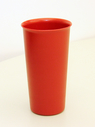
\includegraphics[scale=\examplepicsize]{figures/objects/7.JPG} & 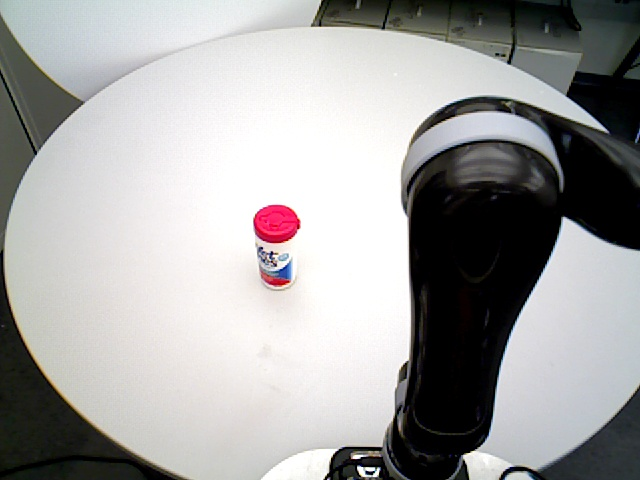
\includegraphics[scale=\examplepicsize]{figures/objects/13.JPG} & 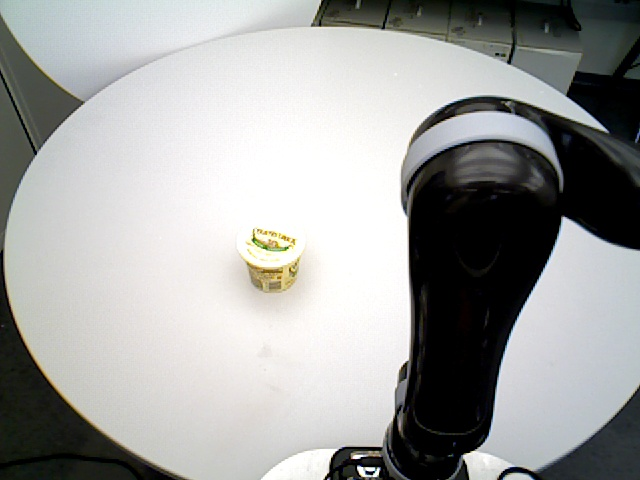
\includegraphics[scale=\examplepicsize]{figures/objects/32.JPG} & 
\includegraphics[scale=\examplepicsize]{figures/objects/31.JPG} & 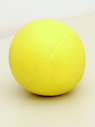
\includegraphics[scale=\examplepicsize]{figures/objects/25.JPG}\\ \hline
	red & -.663 & 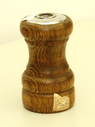
\includegraphics[scale=\examplepicsize]{figures/objects/8.JPG} & 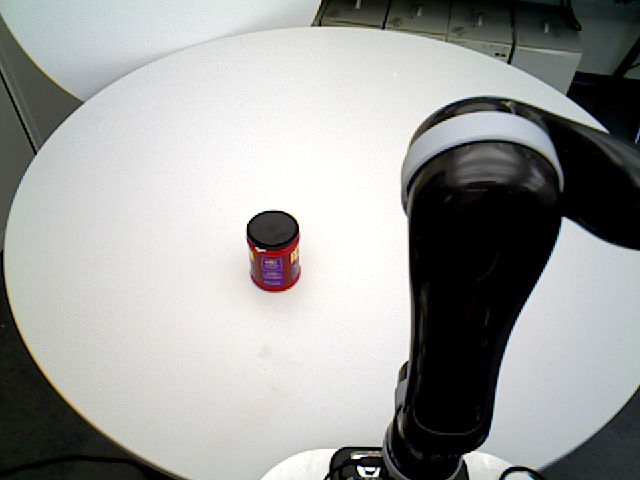
\includegraphics[scale=\examplepicsize]{figures/objects/10.JPG} & 
\includegraphics[scale=\examplepicsize]{figures/objects/14.JPG} & 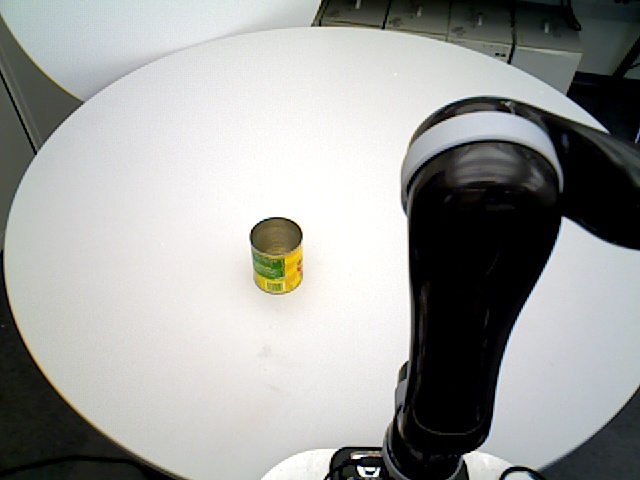
\includegraphics[scale=\examplepicsize]{figures/objects/12.JPG} & 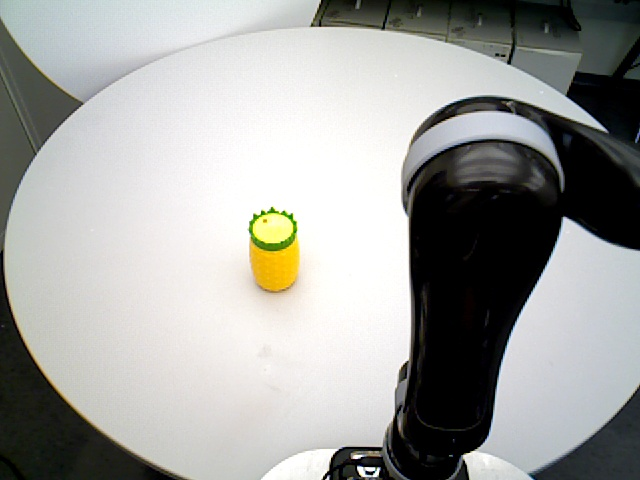
\includegraphics[scale=\examplepicsize]{figures/objects/5.JPG} & 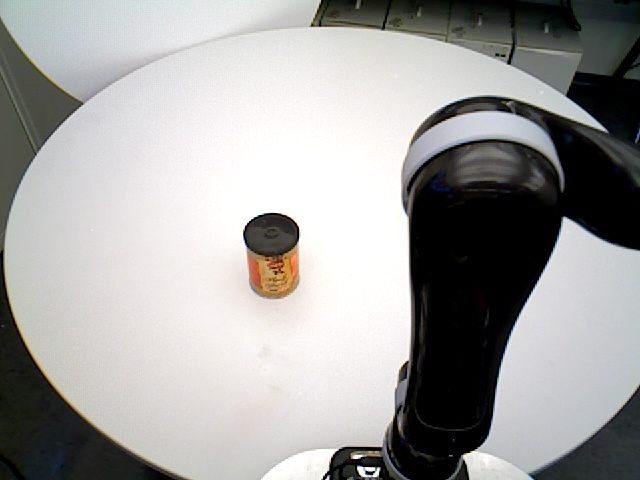
\includegraphics[scale=\examplepicsize]{figures/objects/3.JPG}\\ \hline
	yellow & -1 & 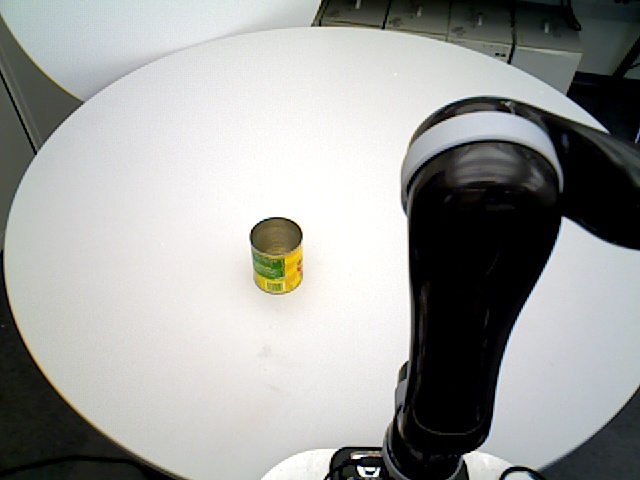
\includegraphics[scale=\examplepicsize]{figures/objects/12.JPG} & 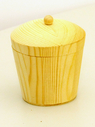
\includegraphics[scale=\examplepicsize]{figures/objects/20.JPG} & 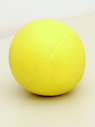
\includegraphics[scale=\examplepicsize]{figures/objects/25.JPG} & 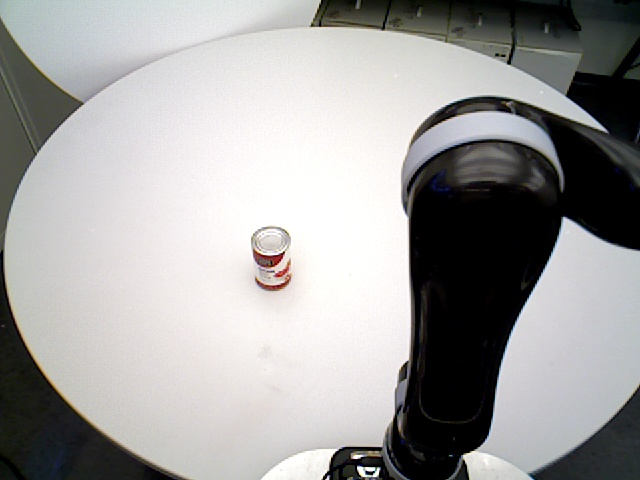
\includegraphics[scale=\examplepicsize]{figures/objects/1.JPG} & \includegraphics[scale=\examplepicsize]{figures/objects/4.JPG} & \includegraphics[scale=\examplepicsize]{figures/objects/17.JPG}\\ \hline
\end{tabular}
\caption{Predicates for which the difference $|\kappa_{mm}-\kappa_{vo}|$ between the \textbf{multi-modal} (mm) and \textbf{vision only} (vo) systems was greater than $0.5$ and both systems had at least $10$ objects with labels for that predicate on which to train.}
\label{tab:predicate_examples}
\end{table*}

The predicates with the highest differences in which the \textbf{multi-modal} system are ``can'' and ``tub'', for which it achieves total agreement with human labels.
The \textbf{vision only} system, on these predicates, classified all objects as not having these properties, a decision that rewards $\kappa=0$.
The reverse happens for color predicate ``yellow,'' except \textbf{multi-modal} eagerly classified all objects as yellow and earned $\kappa=0$.
We note that ``can'' and ``tub'' are cases of instance recognition, for which visual data is certainly helpful but the non-visual of an object could help (e.g. cans are light, tubs are heavy).
In contrast, ``yellow'' is a color word for which only visual properties can help, and the additional noise from other contexts was enough to overwhelm the \textbf{multi-modal} approach.

More interesting cases lie between, where non-trivial classifier decisions were made.
Predicates ``empty'' and ``tall'' have clear non-visual interpretations.
An empty object will be light, while a tall object will exert force earlier against an arm pressing down on it.
The color predicate ``red'' follows the same reasoning as ``yellow'', where non-visual information can serve only to confuse a grounding system.
The ``small'' predicate is a surprise, since a signal inverse to what gives \textbf{multi-modal} an advantage for ``tall'' should do the same for short, small objects.
A possible but uninteresting explanation is that the \textbf{vision only} system has about 1.5 times the labels of \textbf{multi-modal} for this predicate.

\paragraph{Correlations to objective measures.}
To validate whether the systems are learning non-visual properties of objects, for every predicate we calculated the Pearson's correlation $r$ between its signed confidence in whether each object did or did not have the property and that object's measured weight, height, and width. Table~\ref{tab:predicate_correlations} gives the correlations discovered with both high coefficient $r$ and high statistical confidence.

\begin{table}
\centering
\begin{tabular}[h]{|l|r|r|}
	\hline
	\bf Property & \bf multi-modal & \bf vision only \\ \hline \hline
	& \multicolumn{2}{c|}{\bf Believable} \\ \hline
	\bf height & tall (.739) & heavy (.729) \\ \hline
	\bf width & fat (.509) & small (-.525) \\ \hline
	\bf weight & empty (-.771) & \\ \hline \hline
	& \multicolumn{2}{c|}{\bf Likely spurious} \\ \hline
	\bf width & & rattles \\ \hline
	& water, blue & \\
	\bf weight & silver, liquid & \\ 
	& gray, red, yellow & \\ \hline

\end{tabular}
\caption{Predicates and associated Pearson's correlation coefficient $r$ between systems' object decisions and physical object properties.
Shown here are predicates for which $r>0.5$ with $p<0.05$ and the system had at least $10$ objects with labels for the predicate on which to train.}
\label{tab:predicate_correlations}
\end{table}

The \textbf{vision only} system seems able to ground ``heavy'' in height and ``small'' in width, the latter of which is a visual word-property pair (``heavy'' for height has counter-examples in our dataset).
The system can represent these shape properties with the vision features associated with the pointcloud.

In contrast, the \textbf{multi-modal} system learned to ground predicates which correlate well to each of the physical dimensions along which we measured objects.
The ``tall'' predicate correlates with objects that have a high height, ``fat'' with objects that have a high width, and ``empty'' with objects that weigh less.
This highlights the value of multi-modal grounding, since words like ``empty'' cannot be evaluated with vision alone when dealing with containers that have un-seeable contents.

\section{Conclusion}
\label{sec:conclusion}
We expand past work on grounding natural language in robot sensory perception by going beyond vision and exploring haptic, auditory, and proprioceptive robot senses.
We compare a vision only grounding system to one that uses these additional senses by employing an embodied robot playing \ispy with many human users.
To our knowledge, ours is the first robotic system to perform natural language grounding using multi-modal sensory perception through natural interaction with human users.

We demonstrate quantitatively, through the number of turns the robot needs to guess objects described by humans, as well as through agreement with humans on language predicate labels for objects, that our multi-modal framework learns more effective lexical groundings than one using vision alone.
We also explore the learned groundings qualitatively, showing words for which non-visual information helps most as well as when non-visual properties of objects correlate with learned meanings (e.g. ``empty'' correlate negatively with object weight).

In the future, we would like to use one-class classification methods to remove the need for a follow-up dialog asking about particular predicates applied to an object to gather negative labels.
Additionally, we would like to detect polysemy for predicates whose meanings vary across sensory modalities.
For example, the word ``light'' can refer to weight or color.
Our current system fails to distinguish these senses, while human participants intermix them.


% \section*{Acknowledgments}

%% The file named.bst is a bibliography style file for BibTeX 0.99c
\clearpage
\bibliographystyle{named}
\bibliography{/u/ml/bib/lunar,/u/jesse/local}

\end{document}
